\Section{Code Malleability: A Case Study}
\label{section:chroma}

A noteworthy aspect of the StreamIt implementation is its
malleability. We illustrate this by outlining how the decoder
implementation is modified to support both 4:2:0 and 4:2:2 chroma
formats. MPEG-2 streams are typically encoded using the former, which
achieves a 50\% reduction in the number of blocks required to
represent a video. However, better quality is possible with higher
sampling rates since more color information is retained from the
original picture. In this section, we show that the migration path is
trivial.

%% To illustrate the concrete benefits of programming in a stream
%% language, we compare the support for varying chroma formats in the
%% StreamIt and C implementations.  While
The conceptual difference between chroma formats is merely a change in
downsampling ratio. The change affects the data I/O rates, and the
ratios of data between color channels. In the C reference code, the
change requires adjustments to buffer sizes, array lengths, array
indices, and various pointer offsets. The reference implementation
uses a \texttt{chroma flag} to dictate control flow and alternate
index/offset calculations in 43 locations in the code. As an example,
Figure~\ref{fig:chroma-format-code} shows a code fragment from the
\texttt{form\_prediction} routine in
\texttt{recon.c}~\cite{reference-mpeg-c}. The function calls a
subroutine to perform the motion compensation on each of the three
color channels, passing in array offsets to a global array holding the
data. Lines 4-6 adjust values used for address calculations to handle
the 4:2:2 and 4:2:0 chroma formats, and lines 7-9 provide additional
adjustments for the 4:2:0 format. While these offset adjustments are
necessary in C, they are difficult for programmers and make the code
hard to understand.

To add support for the 4:2:2 chroma format in our StreamIt decoder, we
modified 31 lines and added 20 new lines. Of the 31 modified lines, 23
were trivial modifications to pass a variable representing the chroma
format as a stream parameter. The greatest substantial change was to
the color channel splitter, previously illustrated on line 24 of
Figure~\ref{fig:dec-with-code}. In the case of a 4:2:2 sampling rate,
the chrominance data, as they appear on the input tape, alternate
between each of the two chrominance channels (see
Figure~\ref{fig:chroma-block-layout}). Thus, a nested splitjoin is used
to properly recover the chrominance channels. The new splitjoin is
shown on the right half of Figure~\ref{fig:chroma-format-code}.  In
the StreamIt code, the chroma format explicitly dictates control flow
in only 9 locations. Of course, the scheduling and buffer management
changes dramatically between chroma formats, but this is transparent
to the programmer.

\begin{figure*}[t]
 \begin{minipage}[t]{4.3in}{
  \begin{scriptsize}
   \begin{verbatim}
   01 /* Y */
   02 form_component_prediction(src[0]+(sfield?lx2>>1:0),dst[0]+(dfield?lx2>>1:0),
   03                           lx,lx2,w,h,x,y,dx,dy,average_flag);
   04 if (chroma_format!=CHROMA444)  {
   05    lx>>=1; lx2>>=1; w>>=1; x>>=1; dx/=2;
   06 }
   07 if (chroma_format==CHROMA420)  {
   08    h>>=1; y>>=1; dy/=2;
   09 }
   10 /* Cb */
   11 form_component_prediction(src[1]+(sfield?lx2>>1:0),dst[1]+(dfield?lx2>>1:0),
   12                           lx,lx2,w,h,x,y,dx,dy,average_flag);
   13 /* Cr */
   14 form_component_prediction(src[2]+(sfield?lx2>>1:0),dst[2]+(dfield?lx2>>1:0),
   15                           lx,lx2,w,h,x,y,dx,dy,average_flag);    
   \end{verbatim}
  \end{scriptsize}
 }
 % \caption{C code exerpt for handling 4:2:0 and 4:2:2 chroma formats.}
 \label{fig:chroma-stream}
 \end{minipage}
 ~~\vrule~~
 \begin{minipage}[t]{4.3in}{
  \begin{scriptsize}
   \begin{verbatim}
   // C = blocks per chrominance channel per macroblock 
   // C = 1 for 4:2:0, C = 2 for 4:2:2
   add splitjoin {
      split roundrobin(4*(B+V), 2*C*(B+V));
      add MotionCompensation() to PT1;
      add splitjoin {
         split roundrobin(B+V, B+V);
         for (int i = 0; i < 2; i++) {
            add MotionCompensation() to PT1;
            add ChannelUpsample(C);
         }
         join roundrobin(1, 1);
      }
      join roundrobin(1, 1, 1);
   }
   \end{verbatim}
  \end{scriptsize}
 }
 % \caption{StreamIt code exerpt for handling 4:2:0 and 4:2:2 chroma formats.}
 % \label{fig:chroma-stream}
 \end{minipage}
 \caption{C (left) and StreamIt (right) code exerpts for handling
          4:2:0 and 4:2:2 chroma formats.} % during motion compensation.}
 \label{fig:chroma-format-code}
\end{figure*}

\begin{figure}[t]
\begin{center}
  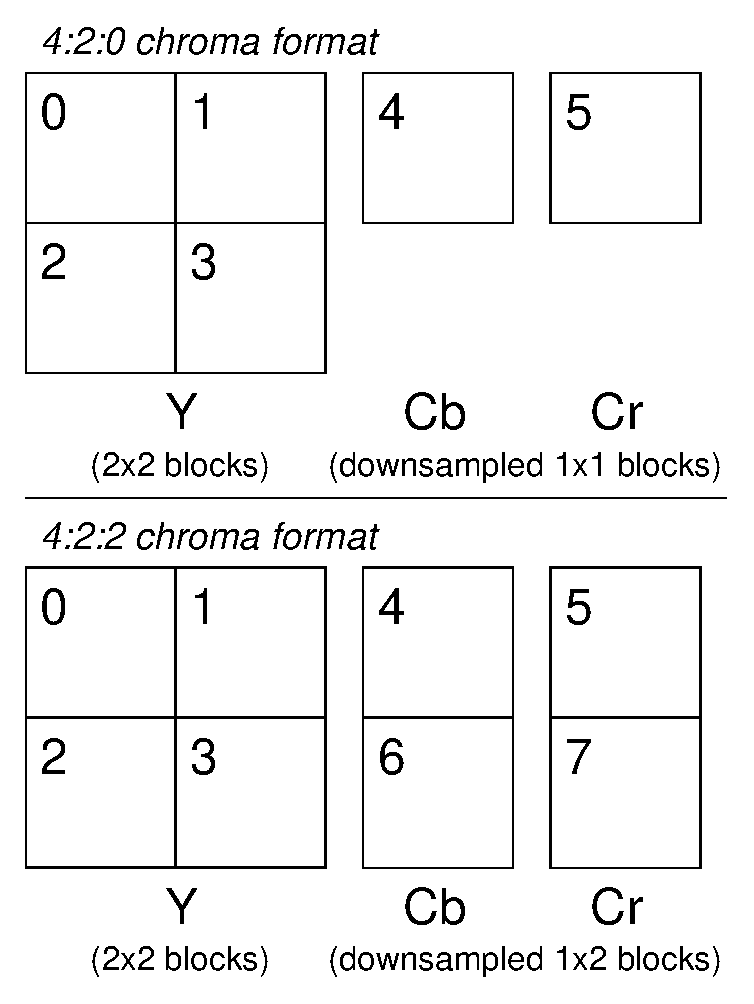
\epsfig{file=chroma_format.eps, width=1.5in}
   \caption{4:2:0 and 4:2:2 chroma formats showing macroblock ordering}
   \label{fig:chroma-block-layout}
\end{center}
\end{figure}